\documentclass[12pt,oneside]{book}
\newcommand{\TITLE}{Thermodynamique}
\usepackage[utf8]{inputenc}
\usepackage[margin=0.5in]{geometry}
\usepackage[usestackEOL]{stackengine}
\usepackage{amsmath , esint,braket,lmodern,mhchem,bohr,lewis,chemfig,draftwatermark,xcolor,graphicx , amssymb ,ragged2e , listings , siunitx , float , eqparbox, centernot , esvect , bm , fancyhdr , fourier-orns}
\usepackage[ddmmyyyy]{datetime}
\usepackage{fourier-orns}
\usepackage{changepage}
\usepackage{bbm}\usepackage{chngcntr}
\usepackage{hyperref}
\usepackage{ifthen}
\usepackage[many]{tcolorbox}
\DeclareMathOperator{\sech}{sech}
\DeclareMathOperator{\csch}{csch}
\DeclareMathOperator{\arcsec}{arcsec}
\DeclareMathOperator{\arccot}{arcCot}
\DeclareMathOperator{\arccsc}{arcCsc}
\DeclareMathOperator{\arccosh}{arcCosh}
\DeclareMathOperator{\arcsinh}{arcsinh}
\DeclareMathOperator{\arctanh}{arctanh}
\DeclareMathOperator{\arcsech}{arcsech}
\DeclareMathOperator{\arccsch}{arcCsch}
\DeclareMathOperator{\arccoth}{arcCoth} 
\DeclareMathOperator{\grad}{\vv{\text{grad}}} 
\DeclareMathOperator{\conj}{^*} 
\DeclareMathOperator{\vect}{vv} 
\DeclareMathOperator{\Vect}{\text{Vect}} 
\DeclareMathOperator{\degree}{c^\circ} 
\DeclareMathOperator{\degre}{^\circ} 
\DeclareMathOperator{\transpose}{^\dagger} 
\DeclareMathOperator{\adjoint}{^\dagger} 

\newcommand{\moyenne}[1]{\langle #1 \rangle} 
\newcommand{\lagrange}{\mathcal{L}}
\newcommand{\fourier}{\mathcal{F}}
\newcommand{\hilbert}{\mathcal{H}}
\newcommand{\p}{\mathcal{P}}
\newcommand{\x}{\chi}
\newcommand{\ve}[1]{\vv{#1}}
\newcommand{\push}[1]{\begin{adjustwidth}{5mm}{}#1\end{adjustwidth}}
\newcommand{\operator}[1]{\widehat{#1}}
\newcommand{\HRule}{\rule{\linewidth}{0.5mm}} % Defines a new command for the horizontal lines, change thickness here
\renewcommand{\chaptermark}[1]{\markboth{\MakeUppercase{#1}}{}}
\renewcommand{\headrule}{%
\vspace{-8pt}\hrulefill
\raisebox{-2.1pt}{\quad\decofourleft\decotwo\decofourright\quad}\hrulefill}
\definecolor{myred}{RGB}{255, 14, 0}
\everymath{\displaystyle}

\def\changemargin#1{\list{}{\leftmargin#1}\item[]}
\let\endchangemargin=\endlist 

\makeatletter
\newcommand*{\rom}[1]{\expandafter\@slowromancap\romannumeral #1@}%roman numbers
\makeatother

%hyperlink shit

\hypersetup{
    colorlinks,
    citecolor=black,
    filecolor=black,
    linkcolor=black,
    urlcolor=black
}
% Table specail cell , it's for making line break in table cell
\newcommand{\specialcell}[2][c]{%
  \begin{tabular}[#1]{@{}c@{}}#2\end{tabular}}

  \definecolor{main}{HTML}{5989cf}    % setting main color to be used
\definecolor{sub}{HTML}{cde4ff}     % setting sub color to be used

\tcbset{
    sharp corners,
    colback = white,
    before skip = 0.2cm,    % add extra space before the box
    after skip = 0.5cm      % add extra space after the box
}   
\newtcolorbox{boxH}{
    colback = sub, 
    colframe = main, 
    boxrule = 0pt, 
    leftrule = 6pt % left rule weight
}
\newtcolorbox{gpt}{
    sharpish corners, % better drop shadow
    boxrule = 0pt,
    toprule = 4.5pt, % top rule weight
    enhanced,
    fuzzy shadow = {0pt}{-2pt}{-0.5pt}{0.5pt}{black!35} % {xshift}{yshift}{offset}{step}{options} 
}
\definecolor{codegreen}{rgb}{0,0.6,0}
\definecolor{codegray}{rgb}{0.5,0.5,0.5}
\definecolor{codepurple}{rgb}{0.58,0,0.82}
\definecolor{backcolour}{rgb}{0.95,0.95,0.92}

\lstdefinestyle{mystyle}{
    backgroundcolor=\color{backcolour},   
    commentstyle=\color{codegreen},
    keywordstyle=\color{magenta},
    numberstyle=\tiny\color{codegray},
    stringstyle=\color{codepurple},
    basicstyle=\ttfamily\footnotesize,
    breakatwhitespace=false,         
    breaklines=true,                 
    captionpos=b,                    
    keepspaces=true,                 
    numbers=left,                    
    numbersep=5pt,                  
    showspaces=false,                
    showstringspaces=false,
    showtabs=false,                  
    tabsize=2,
    basicstyle = \small
}

\lstset{style=mystyle}
\SetWatermarkAngle{45} 
\SetWatermarkLightness{.99} 
\SetWatermarkFontSize{0.1cm} 
\SetWatermarkScale{0} 
\SetWatermarkText{supahaka}


\begin{document}
\pagestyle{fancy}
\fancyhf{}
\fancyfoot[R]{Tenji$_\text{org}$}
\fancyfoot[C]{\thepage}
\fancyfoot[L]{\tiny www.tenji.org}
\fancyhead[RO]{\nouppercase{\leftmark\hfill\TITLE}}


\DraftwatermarkOptions{stamp=false}
    \begin{titlepage}
        \begin{center}
            \vspace*{5cm}
            \Huge
            \HRule \\[0.4cm]
            \textbf{Project Tenji: \\ \TITLE}\\
            \Large 
            \HRule \\[1.5cm]
            \vspace{2cm}
            \vfill
        \end{center}
        \vfill
        { \scriptsize Project Tenji \copyright 2024 by Khalil Salahat and Mohamad El Moussawi  \\}
        { \scriptsize Hosted at tenji.org , contact : contact@tenji.org \\}
        { \scriptsize \NOTICEE  \\}
    \end{titlepage} 
    \tableofcontents
\DraftwatermarkOptions{stamp=true}

\chapter{Premier principe de la thermodynamique}
\section{Definitions}
\begin{itemize}
    \item Thermodynamique : C'est le lien entre les phénomènes thermiques et les phénomènes dynamiques .
    \item Variables thermodynamique : Sont des grandeurs mesurables comme (P,V,T ..).
    \item Energie : C'est la capacité de produire un travail.
\end{itemize}
\section{Chaleur}
La chaleur est l’énergie échangée lors d'un transfert thermique vers ou depuis un système thermodynamique.\\
\begin{itemize}
    \item En variation du temperature la chaleur est :
          \[\boxed{\Delta Q = mc\Delta \theta}\]
          Avec c est la capacité calorifique, $\theta $ est la temperature.
    \item En changement d’état est :
          \[\boxed{\Delta Q = ml}\]
          Avec l est la chaleur latent (Enthalpie de changement d'état).
\end{itemize}
\begin{itemize}
    \item $\Delta Q > 0  \implies $ System reçoit de chaleur
    \item $ \Delta Q < 0 \implies $ System donne de chaleur
\end{itemize}
Note que :
\begin{itemize}
    \item Un changement du temperature n'est pas nécessairement du a un transfer du chaleur .\\
          exemple :\\
          L'augmentation du pression dans un milieu adiabatique
    \item Un Transfer du chaleur n'est pas nécessairement du a un changement du temperature . \\
          exemple : \\
          Fusion de l'eau.
\end{itemize}
\subsection{Transfer de la Chaleur}
\begin{itemize}
    \item Par conduction :\\
          Le transfer de la chaleur par conduction est le déplacement de la chaleur sans déplacement de la matier.La quantité de chaleur qui traverse un surface S pendant dt entre x et x+dx est :\\
          \[\boxed{\frac{\delta Q}{dt} = -kS\frac{d\theta}{dx}}\]
          Avec k est la conductivité thermique .
    \item Convection :\\
          C'est le déplacement de chaleur par déplacement de la matière .
    \item Rayonnement :\\
          C'est le déplacement de chaleur par les rayons électromagnétiques
\end{itemize}
\section{Travail}
Le travail d'une force est l'énergie fournie par cette force lorsque son point d'application se déplace .\\
On a plusieurs type de travail :
\begin{itemize}
    \item Travail mécanique :\\
          \[\boxed{\delta w = |F|dx = -PdV}\]
          Avec P est la pression , V est le volume .
    \item Travail électrique : \\
          \[\delta w = Pdt\]
          avec $P = U\times I$ est la puissance.
    \item Travail diélectrique : \\
          \[\delta w = \vv{E} d\vv{P}\]
          avec P vecteur de polarisation
    \item Travail magnétique :\\
          \[\delta w = B dM\]
          avec B est le champ magnétique et dM est la variation de l'aimantation
\end{itemize}
On note que
\begin{itemize}
    \item Le system reçu de travail lorsque :$\delta w > 0$.
    \item Le system donne de travail lorsque : $\delta w < 0$.
\end{itemize}
\begin{center}
    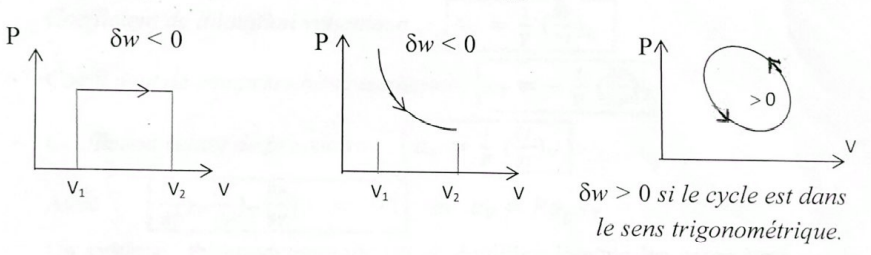
\includegraphics[width=0.8\linewidth]{../pic/3300/1.png}
\end{center}
\section{Type des variables}
\begin{itemize}
    \item Extensive :\\
          Les variables extensive a un caractère additif, c-a-d si le système est multiplié par un nombre K, le variable est multiplié k. (example addition des volumes ..)
    \item Intensive : \\
          les variables qui ne contiennent pas un caractère d'additif comme la (temperature , la pression ...)
\end{itemize}
\section{Système}
\begin{itemize}
    \item Système Ferme : \\
          C'est un système sans changement de matier .
    \item Système Isole : \\
          C'est un system sans changement de matier et l’énergie .
\end{itemize}
\section{Coefficients Thermo-élastiques}
\begin{itemize}
    \item Coefficient de dilatation volumique : \\
          \[\alpha_V =\frac{1}{V}(\frac{\partial V}{\partial T})_P\]
          ($_P : $ a pression constant)
    \item Coefficient de compressibilité isotherme :\\
          \[k_T = \frac{-1}{V}(\frac{\partial V}{\partial P})_T\]
          ($_T :$ a temperature constant )
    \item Coefficient relatif de pression :\\
          \[\alpha_P=\frac{1}{P}(\frac{\partial P}{\partial T})_V\]
          ( $_V : $ a volume constant)
\end{itemize}
On a la propriétés suivant :
\[\boxed{\frac{\partial V}{\partial T})_P \frac{\partial T}{\partial P})_V\frac{\partial P}{\partial V})_T = -1 }\]
$\text{ et } \alpha_V = P\alpha_pk_T $\\
\underline{Preuve :}
on a $f(T,V,P) = cte \implies df = 0$ \\
$df = \frac{\partial f}{\partial T}dT + \frac{\partial f}{\partial P}dP + \frac{\partial f}{\partial V}dV = 0$ \\
\begin{itemize}
    \item a $T = cte \implies dT = 0$\\
          $\frac{\partial f}{\partial V}dV = -\frac{\partial f}{\partial P}dP \implies \frac{dV}{dP})_T = \frac{\frac{-\partial f}{\partial P}}{\frac{\partial f}{\partial V}}$
    \item a $V =cte \implies dV =0$\\
          $\frac{\partial f}{\partial T} dT = \frac{-\partial f}{\partial P}dP \implies \frac{dT}{dP})_T = \frac{\frac{-\partial f}{\partial p}}{\frac{\partial f}{\partial T}} $
    \item a $P = cte \implies dP = 0$\\
          $\frac{\partial f}{\partial T}dT = -\frac{\partial f dV}{\partial V}dV \implies \frac{dV}{dT})_T = \frac{-\frac{\partial f}{\partial T}}{\frac{\partial f}{\partial V}}$
\end{itemize}
$\implies \frac{\partial V}{\partial T})_P \frac{\partial T}{\partial P})_V\frac{\partial P}{\partial V})_T = -1$
\section{l’équilibre }
Un system thermodynamique est en équilibre lorsque les paramètres qui le caractérisent , a l’échelle macroscopique , ne varient pas au cours du temps.
\section{Transformation}
\begin{itemize}
    \item Adiabatique : sans échange de chaleur avec l’extérieur .
    \item Isotherme : la temperature du système reste constante .
    \item Isobare : la pression reste constante .
    \item Isochore : le volume reste constant .
\end{itemize}
\section{Zero principe de la thermodynamique }
\begin{center}
    \underline{Deux systemes en equilibre thermique avec un troisieme sont en equilibre thermique entre eux .}
\end{center}
\section{Premier principe de la thermodynamique}
\begin{center}
    \underline{L'énergie se conserve, elle ne peut être ni créée, ni détruite, elle ne peut que se transformer.}
\end{center}
Le principe introduit une énergie U appelé énergie interne du système qui est la somme de son énergie cinétique et potentille a l’échelle microscopique, en l’absence du transfer du matière on a :
\[\boxed{\Delta U = \delta w + \delta Q}\]
\begin{itemize}
    \item U est variable d’état
    \item U independent du chemin suivit
    \item $\Delta U = 0$
          \begin{itemize}
              \item L'ors d'un cycle
              \item Pour un system isole
          \end{itemize}
\end{itemize}
\chapter{Gaz parfait}
\section{Definition}
Un gaz parfait est un modèle thermodynamique décrivant le comportement des gaz réels à basse pression.
\section{Lois de base}
\begin{minipage}{0.7\linewidth}
    Soit une bois qui contient un gaz parfait monoatomique .\\
    Volume :V = $l_xl_yl_z$.\\
    La masse s'une particule : m . \\
    Vites du particule : $\vv{v} = (v_x,v_y,v_z)$
\end{minipage}
\begin{minipage}{0.3\linewidth}
    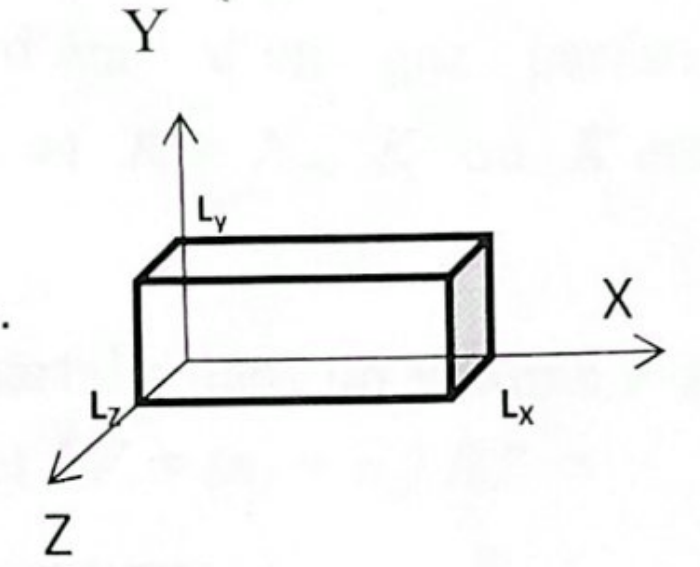
\includegraphics[width=\linewidth]{../pic/3300/2.png}
\end{minipage}
\begin{itemize}
    \item La particule frap le plan $l_yl_z$ a $x=0$ puis elle march $l_x$ et frap le plan $l_yl_z$ a $x = l_x$ et elle remarcha $l_x$ pour refrappé le plan $l_yl_z$ a $x=0$.\\
          Lors d'une collision élastique d'une particule avec la paroi $l_y l_z$ :
          \begin{itemize}
              \item Le moment cinétique selon x :$\Delta P_x = 2mv_x$
              \item Le temp qui sépare deux collision: $\Delta t = \frac{2 l_x}{v_x}$
          \end{itemize}
    \item L'equation fondamentale de la dynamique : $F= \frac{dP}{dt}$\\
          $\implies F_x =\frac{\Delta P_x}{\Delta t}=\frac{2mv_x^2}{2l_x} = 2 \frac{\moyenne{\varepsilon}}{3l_x}$Avec $\varepsilon = \frac{1}{2}mv^2$ (l’énergie cinétique)
    \item Pour N particule : $F = 2 N \frac{\moyenne{\varepsilon}}{3l_x}$
    \item Alors la pression sur cette paroi :\\
          $P =\frac{F}{S} = 2N \frac{\moyenne{\varepsilon}}{3l_xl_yl_z} = 2\frac{N\moyenne{\varepsilon}}{3V}$\\
          \[\boxed{P = \frac{2U}{3V}}\]
          Avec U est l’énergie interne du système.
\end{itemize}
\section{Lois relative au gaz parfait}
\begin{itemize}
    \item L'expression des gaz parfait :
          \begin{itemize}
              \item Loi de Boyle-Mariotte :\\
                    A une  temperature constant :
                    \[P.V = cte\]
              \item Loi d'Avogadro : \\
                    Des volumes égaux de gaz parfait , a la meme temperature , a la meme pression , contiennent le meme nombre de moles.
              \item Loi de Gay-Lussac : \\
                    A P constant , le rapport $\frac{V}{T}$ est constant avec T en kelvin
              \item Loi de Charles :\\
                    A V constant ,le rapport $\frac{P}{T}$ est constant avec T en kelvin .
          \end{itemize}
          D'apres les lois precedent :
          \[\boxed{PV = nRT}\]
          Avec :$\begin{cases}
                  R= N_{av}K = 8.31                                             \\
                  K = 1.38\times 10^{-23} \text{ est la constant de boltzmann.} \\
                  N_{av} \text{ est le nombre d'avogadro.}
              \end{cases}$

    \item Loi de Dalton :  Soit un melange de 2 gas parfaits dans un volume V a la temperature T . \\
          $P_1V = n_1RT$ et $P_2V =n_2RT $ et $PV = (n_1 + n_2)RT \implies \frac{P_1}{n_1} = \frac{P_2}{n_2} = \frac{P}{n_1 + n_2}$
          \[ \boxed{ P = P_1 + P_2} \]
    \item Loi de Joule :\\
          D'apres le loi de Base :$U = \frac{3}{2}PV$\\
          D'apres l'expression des gaz parfaite :$PV =nRT=(N/N_{av})N_{av}KT = NKT$
          \[\boxed{U = \frac{3}{2}NKT}\]
\end{itemize}
\section{Enthalpie}
L'enthalpie joue pour les transformations à pression constante, le rôle que joue l'énergie interne pour les transformations à volume constant.
\[\boxed{H = U + PV}\]
Pour les processus effectués à pression constante, la variation d'enthalpie correspond à la chaleur absorbée (ou dégagée) pour rester à température constante :
\[\Delta H = Q_p = \Delta U + P\Delta V\]
\section{Capacité calorifique}
La capacité calorifique est la quantité de chaleur qu'il faut fournir pour élever de un degré la température d'une substance.\\
On définit deux grandeurs macroscopiques que sont les capacités calorifiques:
\begin{itemize}
    \item à pression constant :
          \[\boxed{C_V = \frac{dU}{dT} = \frac{\partial U}{\partial T}_V}\]
    \item à volume constant :
          \[\boxed{C_P =\frac{dH}{dT} =  \frac{\partial H}{\partial T}_P}\]
\end{itemize}
Dan le grandeur molaire :
\begin{itemize}
    \item $C_{V_m} = \frac{C_P}{n} = \begin{cases}
                  \text{Pour un gaz monoatomique :} C_{V_m} = \frac{3}{2}R \\
                  \text{Pour un gaz diatomique :} C_{V_m} = \frac{5}{2}R   \\
                  \text{Pour un gaz polyatomique :} C_{V_m} = \frac{6}{2}R = 3R
              \end{cases}$
    \item $C_{P_m} = \frac{C_P}{n} = R + C_{Vm}$
\end{itemize}
On défini : $\gamma = \frac{C_P}{C_V} = \frac{C_{Pm}}{C_{Vm}}$
\section{Théorème de l’équipartition de l’énergie }
En physique statistique classique, l'équipartition de l'énergie est un résultat remarquable selon lequel l'énergie totale d'un système à l'équilibre thermodynamique est répartie en parts égales en moyenne entre ses différentes composantes.
\begin{center}
    Dans un système à l'équilibre à la température T, chaque degré de liberté contribue pour $1/2k_{B}T$ à l'énergie totale, où $k_{B}$ est la constante de Boltzmann.
\end{center}
\begin{itemize}
    \item Pour un gaz monoatomique : \\
          Un gaz monoatomique posed 3 degré de liberté de translation seulement. \\
          $\implies \varepsilon_i = \frac{1}{2}m_0(v_x^2 + v_y^2 + v_z^2) $ \\
          $\implies U = \moyenne{\varepsilon_i} =\frac{1}{2}KT + \frac{1}{2}KT + \frac{1}{2}KT = \frac{3}{2}KT $ \\
          Pour N particule :\\
          $U = \frac{3}{2}NKT \implies \boxed{C_{Vm} = \frac{3}{2}R}$
    \item Pour un gaz diatomique : \\
          Un gaz diatomique posed 3 degré de liberté de translation et 2 degré de liberté de rotation seulement. \\
          $\implies \varepsilon_i = \frac{1}{2}m_0(v_x^2 + v_y^2 + v_z^2) + \frac{1}{2}I(w_x^2 + w_y^2)$ \\
          $\implies U = \moyenne{\varepsilon_i} =\frac{1}{2}KT + \frac{1}{2}KT + \frac{1}{2}KT + \frac{1}{2}KT + \frac{1}{2}KT = \frac{5}{2}KT $ \\
          Pour N particule :\\
          $U = \frac{5}{2}NKT \implies \boxed{C_{Vm} = \frac{5}{2}R}$
    \item Pour un gaz polyatomique : \\
          Un gaz polyatomique posed 3 degré de liberté de translation et 3 degré de liberté de rotation. \\
          $\implies \varepsilon_i = \frac{1}{2}m_0(v_x^2 + v_y^2 + v_z^2) + \frac{1}{2}I(w_x^2 + w_y^2)+w_z^2$ \\
          $\implies U = \moyenne{\varepsilon_i} =\frac{1}{2}KT + \frac{1}{2}KT + \frac{1}{2}KT + \frac{1}{2}KT + \frac{1}{2}KT + \frac{1}{2}KT = 3KT$ \\
          Pour N particule :\\
          $U = 3NKT \implies \boxed{C_{Vm} = 3R}$
\end{itemize}
\chapter{Second principe de la thermodynamique}
\section{Definition }
\begin{itemize}
    \item Transformation reversible : C'est une transformation ou le système est une suit d’états d’équilibre infiniment voisines
    \item Transformation irréversibles : (n'est pas reversible) , comme les phénomènes suivant :
          \begin{itemize}
              \item Les phénomènes de frottement
              \item Les phénomènes de diffusion (comme melanges de l'eau et sel etc ...)
              \item les échanges de chaleur ( La chaleur est reçu par le système le plus froid )
              \item Les reactions chimiques
          \end{itemize}
\end{itemize}
\section{Second principe de la thermodynamique}
\begin{center}
    La deuxième loi de la thermodynamique affirme qu'il est impossible que la chaleur s'écoule spontanément d'un corps froid vers un corps chaud,
    mais qu'elle peut se déplacer de cette façon si un certain travail est effectué.
\end{center}
\section{L'entropie}
Le terme entropie caractérise le degré de désorganisation.
\begin{itemize}
    \item L'entropie est une grandeur additive
    \item L'entropie reste constant dans une transformation adiabatique reversible
    \item L'entropie augmente strictement dans une transformation adiabatique irreversible
    \item Dans une transformation non adiabatique la variation d'entropie est la somme de deux terme :
          \begin{itemize}
              \item l’échange de chaleur avec l’extérieur
              \item Transformation internes $\begin{cases}
                            > 0 \text{ si irreversible} \\
                            = 0 \text{ si reversible}
                        \end{cases}$
          \end{itemize}
\end{itemize}
\subsection{L'equation différentielle du l'entropie}
Si $\delta Q_e$ est la quantité de chaleur fournie par le milieu extérieur au système , $T$ est la temperature de la source de chaleur , on a :
\[ \boxed{ dS = \frac{\delta Q_e}{T} + dS_i } \]
\begin{itemize}
    \item $dS$ : est la variation d'entropie du système
    \item $dS_i$ : est la creation d'entropie $\begin{cases}
                  > 0 \text{ si irreversible} \\
                  = 0 \text{ si reversible}
              \end{cases}$
    \item $\frac{\delta Q_e}{T}$ : Terme d’échange avec l’extérieur
\end{itemize}
Note que $dS$ est une différentielle totale exacte :elle ne dépend que de l'état initial et de l'état final et non du chemin suivi.\\
En peut écrire dans le cas reversible :
\[\Delta S = \int \frac{\delta Q_{rev}}{T}\]
\section{Cycles thermiques}
\begin{itemize}
    \item Machine diatherme :\\
          C'est la machine la plus simple qui peut fournir un travail au cours d'un cycle .\\
          \begin{minipage}{0.5\linewidth}
              \begin{itemize}
                  \item La machine recevant au cours d'un cycle une quantité de chaleur $\delta Q_1$ d'une source a $T_1$
                  \item La machine fournie un travail (donne de travail)
                  \item La machine donne de chaleur $\delta Q_2$ a une source a $T_2 \text{ ou } T_2<T_1$
              \end{itemize}
          \end{minipage}
          \begin{minipage}{0.5\linewidth}
              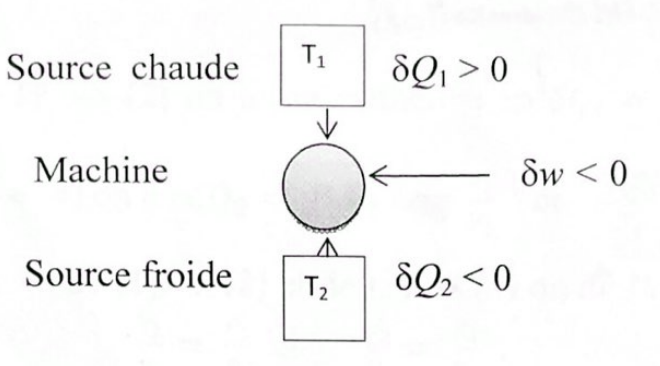
\includegraphics[width=\linewidth]{../pic/3300/3}
          \end{minipage}
          Lorsque $\delta w<0$ , l’efficacité d'une machine est :
          \[\boxed{ \eta = \frac{|\delta w|}{\delta Q_1}  = \frac{\delta Q_1 + \delta Q_2}{\delta Q_1} } \]
    \item Cycle de Carnot : \\
          C'est le moteur idéal , il est réversible, donc il est forcément composé de 2 isothermes et de 2 adiabatiques qui permettent de passer de l'isotherme chaude T2 à l'isotherme froide T1.\\
          Q1 et Q2 sont forcément échangées sur les isothermes puisque les autres transformations n'échangent pas de chaleur. \\
          Calculons l’efficacité :\\
          \begin{minipage}{0.6\linewidth}
              \begin{itemize}
                  \item $1\to 2$ :\\
                        On a un \underline{Isotherme} : $\delta Q_1 = -\delta w = P_1V_1\ln(\frac{V_2}{v_1})$
                  \item $2 \to 3$ : \\
                        On a un \underline{adiabatique} : $P_2V_2^\gamma = P_3V_3^\gamma$
                  \item $3 \to 4$ : \\
                        On a un \underline{Isotherme} : $\delta Q_2 = P_3V_3\ln(\frac{V_4}{V_3})$
                  \item $4 \to 1 :$\\
                        On a un \underline{adiabatique} : $P_4V_4^\gamma = P_1V_1^\gamma$
              \end{itemize}
          \end{minipage}
          \begin{minipage}{0.4\linewidth}
              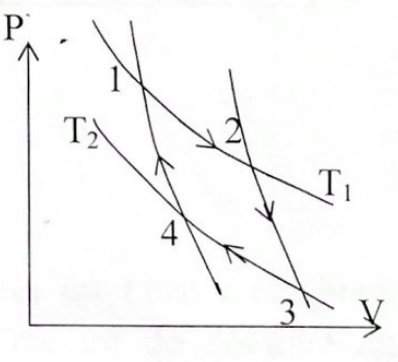
\includegraphics[width=\linewidth]{../pic/3300/4}
          \end{minipage}
          D'apres le premier principe : $W_\text{cycle} = -Q_1 -Q_2$ car $\Delta U_\text{cycle} = 0$\\
          D'apres le second principe : $\Delta S_\text{cycle} -(\frac{Q_1}{T_1}+\frac{Q_2}{T_2} ) = 0$\\
          Puisque la transformation est reversible alors $\Delta S_\text{cycle} = 0 \implies \frac{Q_1}{T_1} + \frac{Q_2}{T_2} = 0$\\
          D'ou $\eta = |\frac{W}{Q_2}| = |\frac{-Q_2-Q_1}{Q_2}| = |-1 - \frac{Q_1}{Q_2}| = |-1 + \frac{T_1}{T_2}| = 1 - \frac{T_1}{T_2}$ \\
          \[\boxed{ \eta = 1 - \frac{T_1}{T_2} }\]
    \item Réfrigérateur : \\
          Ils pompent de la chaleur d'un corps froid et la transmettent à un corps chaud grâce à un compresseur et à un détendeur qui permettent cette opération.
          Ce cycle nécessite de l'énergie motrice (absorption de travail).\\

          \begin{minipage}{0.6\linewidth}
              \begin{itemize}
                  \item La machine absorbe de travail
                  \item La machine donne de chaleur $\delta Q_1$ a une source a $T_1$
                  \item La machine absorbe de chaleur $\delta Q_2$ de source a $T_2$ \underline{ou $T_2 < T_1$}
              \end{itemize}
          \end{minipage}
          \begin{minipage}{0.4\linewidth}
              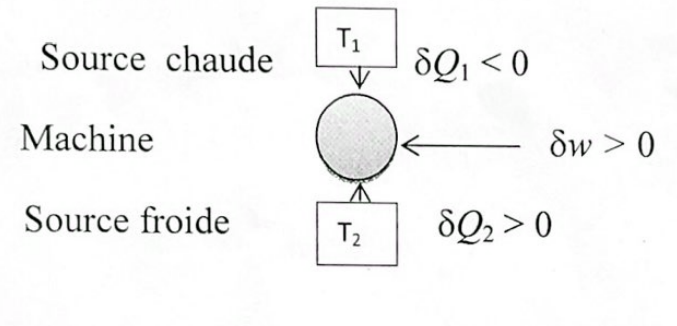
\includegraphics[width=\linewidth]{../pic/3300/5}
          \end{minipage}
          D'apres le premier principe au cours d'un cycle : $\delta Q_1 + \delta Q_2 + \delta w = 0$, l’efficacité : \\
          $\eta_\text{rev} = \frac{\delta Q_2}{\delta w} = \frac{\delta Q_2}{-\delta Q_1-\delta Q_2}$ avec $\frac{\delta Q_2}{\delta Q_1} = - \frac{T_2}{T_1}$
          \[\boxed{ \eta_\text{rev} = \frac{\delta Q_2}{\delta w}=\frac{T_2}{T_1-T_2} }\]
\end{itemize}
\subsection{L'entropie de vue statistique}
L'entropie du système est définie comme une mesure du désordre du système ou du manque d'information.\\
Boltzmann definite l'entropie par $S = -k\sum^M_{m=1}P_m\ln(P_m)$, ou k est la constant de Boltzmann, $P_m$ est la probabilité d'un événement parmi M autres .
\begin{itemize}
    \item S est minimum (null) lorsque l'une des probabilité vaut 1 et les autres null . (l'information est complete)
    \item S est maximum , lorsque les M événement sont équiprobables .
    \item S augmente lorsque M augmente .
\end{itemize}
\chapter{Fonction thermodynamiques Gaz reels}
\section{Relations de Maxwell}
Pour un système entièrement décrit par les grandeurs pression P, température T, entropie S et volume V, on retient généralement un ensemble de quatre relations relatives à l'énergie interne, à l'enthalpie, à l'énergie libre et à l'enthalpie libre :\\
\begin{minipage}{0.5\linewidth}
    \begin{itemize}
        \item $-(\frac{\partial P}{\partial S})_V = (\frac{\partial T}{\partial V})_S$
        \item $(\frac{\partial V}{\partial S})_P = (\frac{\partial T}{\partial P})_S$
        \item $(\frac{\partial P}{\partial T})_V = (\frac{\partial S}{\partial V})_T$
        \item $(\frac{\partial V}{\partial T})_P = -(\frac{\partial S}{\partial P})_T$
    \end{itemize}
\end{minipage}
\begin{minipage}{0.2\linewidth}
    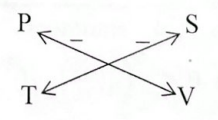
\includegraphics[width=\linewidth]{../pic/3300/6.png}
\end{minipage}

\section{Relation de Helmholtz}
L'énergie libre de Helmholtz est un concept en thermodynamique où le travail d'un système isole avec la température et le volume constants est mesuré en utilisant le potentiel thermodynamique. Il peut être décrit comme l'équation suivante :
\[ F = U -TS \]
\begin{itemize}
    \item $F :$ Helmholtz énergie
    \item $U :$ Energie interne
    \item $T :$ Temperature de l’environnement
    \item $S :$ Entropie
\end{itemize}
\section{Coefficients calorimétriques}
En thermodynamique, les coefficients calorimétriques et thermoélastiques sont des coefficients permettant d'exprimer:
\begin{itemize}
    \item la chaleur absorbée par un système thermodynamique
    \item les variations de volume et de pression de ce système
\end{itemize}
Dans une transformation reversible, la chaleur $Q$ absorbée par un corps pur ou un melange de composition constante peut être exprimée a l'aide de coefficients calorimétriques :
\begin{itemize}
    \item $\delta Q = TdS = C_VdT + ldV$
    \item $\delta Q = TdS = C_PdT + \mathcal{K}dP$
\end{itemize}
avec \begin{itemize}
    \item S : l'entropie
    \item T : la temperature
    \item P : la pression
    \item V : le volume
    \item $C_V =T(\frac{\partial S}{\partial T})_V $ : capacité thermique isochore
    \item $C_p = T(\frac{\partial S}{\partial T})_P:$ capacité thermique isobare
    \item $l = T(\frac{\partial S}{\partial V})_T=T(\frac{\partial P}{\partial T})_V$ : coefficient de dilatation isotherme (chaleur latent)
    \item $\mathcal{K} = T (\frac{\partial S}{\partial P})_T = -T(\frac{\partial V}{\partial T})_P:$ coefficient de compression isotherme
\end{itemize}
Avec l’énergie interne\\
La différentielle de l'énergie interne U si le processus est réversible et si le travail n'est dû qu'aux forces de pression s'écrit :
\[dU = -PdV + TdS\]
en substituant $TdS = C_V dT + ldV$ on obtient :
\[ \boxed{dU = C_VdT+(l-P)dV} \]
Avec l'enthalpie \\
La différentielle de l'enthalpie H si le processus est réversible et si le travail n'est dû qu'aux forces de pression s'écrit :
\[dH = VdP + TdS\]
en substituant $TdS = C_pdT + \mathcal{K}dP$ on obtient :
\[ \boxed{dH = C_pdT + (\mathcal{K}+V)dP} \]
\section{Autre system bivariants}
\begin{itemize}
    \item  Force de traction
          \[\delta w = fdL\]
          Dans ce cas
          \begin{itemize}
              \item la pression $P$ est associe a $f$,$f$ étant la force de traction
              \item $V$ associe a $-L$ ou $L$ est la longueur du fil.
          \end{itemize}
          $dU = TdS + fdL;H = U-fL$
    \item Force électromotrice
          \[\delta w = -Edq\]
          Dans ce cas
          \begin{itemize}
              \item la pression $P$ est associe a $E$ force électromotrice
              \item $V$ associe a $q$ charge débitée.
          \end{itemize}
          On a $\begin{cases}
                  \delta Q = TdS = C_VdT + ldV \\
                  \delta Q = TdS = C_PdT + \mathcal{K}dP
              \end{cases} \implies \boxed{C_P-C_V = T(\frac{\partial P}{\partial T})_V.(\frac{\partial V}{\partial T})_P} $

\end{itemize}



\section{Gaz reels}
Dans la pratique , les gaz reels ne peuvent être représentes par des equation simples que dans un intervalle limite.\\
Pour des domaines plus larges ,la relation entre les variables d’état est établie expérimentalement.\\
Les diagramme les plus commodes sont:
\begin{itemize}
    \item Diagramme d'Andrews:\\
          La diagramme Andrews est la représentation en Plan (P-V) sur le comportement du système gaz-liquide d'une substance.
          \begin{center}
              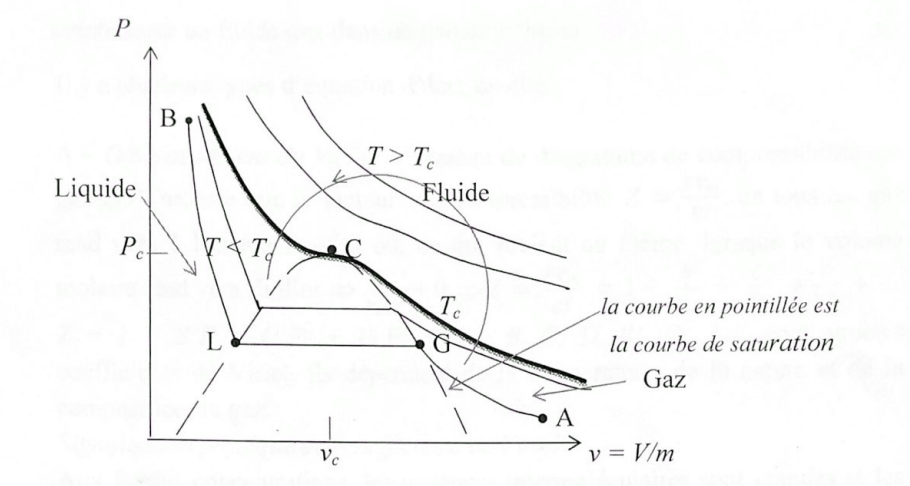
\includegraphics[width=0.6\linewidth]{../pic/3300/7.png}
          \end{center}
          \begin{itemize}
              \item Pour $T < T_C$, l'isotherme présente trois parties :
                    \begin{itemize}
                        \item AG : phase gazeuse
                        \item GL : phase de liquefaction $\implies$ équilibre liquide-gaz du fluide.
                        \item LB : phase liquide seule
                    \end{itemize}
                    Lorsque T augmente LG diminue jusqu'a s'annuler pour $T = T_C$.\\
                    L'ensemble des extrémités LG représente la courbe de saturation.
                    \push{En compression isothereme du fluide , en G apparait la premiere goutte de liquide , en L disparette la derniere bulle de gaz }
              \item  Pour $T > T_C$, les courbes prennent plus une forme hyperbolique.
          \end{itemize}
          Note que :
          \begin{itemize}
              \item En point C les phases liquide et gaz ont les memes propriétés.
              \item Au-dessus de $T_C$, il est impossible de liquefier le gaz pour toute pression.
          \end{itemize}
\end{itemize}
\subsection{Equation d’état des gaz reels}
Il est plus commode de décrire un fluide par une equation d’état que par un reseau d'isothermes.Cependant , les equations d’état ne représentent de façon satisfaisante un fluide que dans un domaine limite.\\
il ya plusieurs types d’équation d’état , on cite :
\begin{itemize}
    \item Développement du Viriel :\\
          L'équation d'état du Viriel est une équation d'état utilisée pour décrire le comportement des fluides.\\
          Elle s'écrit le plus souvent comme l'expression de Z(le facteur de compressibilité) en fonction des puissances de $\frac{1}{V_m}$(le volume molaire) ou en fonction de la pression P  :
          \[\boxed{ Z = 1 + \frac{B}{V_m}+\frac{C}{V_m^2}+\frac{D}{V_m^3}+...=1 + B'P + C'P^2+D'P^3+...} \]
          Les coefficient $B,C,D,B',C',D'...$ est appelé les coefficient du Viriel . les coefficients sont determines expérimentalement pour les fluides reels . \\
          On note le facteur de compressibilité : $\boxed{Z = \frac{PV_m}{RT}}$\\
          Physiquement , le deuxième terme de l'equation de Viriel décrit la déviation par rapport à l'idéalité due aux interactions entre paires de molécules\\
          le troisième terme décrit la déviation due aux interactions entre triplets de molécules.
    \item Equation de Van der Waals : \\
          L'équation d'état de van der Waals fut historiquement une avancée considérable par rapport à l'équation des gaz parfaits, puisque, en plus de décrire le comportement d'un gaz réel plus précisément que le modèle des gaz parfaits.\\
          L'equation :
          \[ \boxed{(P + \frac{an^2}{V^2})(V-nb) = nRT} \]
          avec :
          \begin{itemize}
              \item $a$ : le terme de cohesion (constant)
              \item $b$ : le covolume molaire (constant)
              \item $n$ : nombre de moles
          \end{itemize}
\end{itemize}
\chapter{Équilibre et stabilité des système thermodynamiques}
\section{En mécanique}
L'énergie mécanique $E_m$ d'un système, soumis seulement à des forces qui dérivent d'une énergie potentielle $E_p$, se conserve, ce que l'on traduit par l'équation :
\[ E_m = E_c + E_p = cte \]
Pour un système mécanique soumis a des forces qui dérivent d'une énergie potentielle $\begin{cases}
        E_c : \text{ Energie cinetique } \\
        E_p : \text{ Energie potentielle }
    \end{cases}$
\begin{itemize}
    \item La condition d'evolution : $dE_p \leq 0$
    \item La condition d’équilibre : $(\frac{dE_p}{dq})_\text{eq} = 0$
    \item La condition de stabilité : $(\frac{d^2E_p}{dq^2})_\text{eq} > 0$
\end{itemize}
\section{L'entropie}
Pour un System thermodynamique isole ona :
\[ \Delta S \geq 0 \]
L'entropie ne peut qu'augmenter, ou (- S) ne peut que décroître ; par analogie avec la mécanique et l'énergie potentielle (qui est minimale en une position d'équilibre stable), (- S) représente un potentiel thermodynamique pour un système isolé.\\
Un état d’équilibre correspond a un maximum de S (minimum de -S) pour une énergie interne constant donne:
\begin{center}
    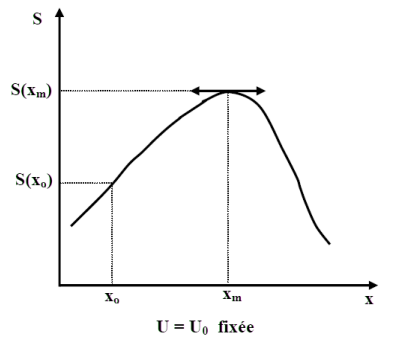
\includegraphics[width=0.5\linewidth]{../pic/3300/8.png}
\end{center}
Mais l'emploi de ce potentiel est rarement intéressant car les systèmes réels échangent le plus souvent matière et énergie avec l'extérieur.
\section{Potentiel thermodynamique}
On appelle potentiel thermodynamique d'un système soumis à un certain nombre de contraintes, toute fonction qui décroît au cours de l'évolution spontanée du système, l'équilibre thermique correspondant à son minimum. \\
Examples
\begin{itemize}
    \item Système mécanique : énergie potentielle.
    \item Système fermé thermodynamiquement isolé : néguentropie -S.
    \item Evolution monotherme  et isochore : potentiel F.\\
          F est l’énergie libre (énergie de Helmholtz)
          \[F = U - TS\]
          la variation de la fonction F est égale au travail fourni par le système si la transformation est effectuée à T constante et si elle est réversible.
    \item Evolution monotherme  et monobare : potentiel G.\\
          G est l'enthalpie libre (énergie libre de Gibbs) :
          \[G = H-TS\]
          \[G =U+PV-TS\]
          Le changement d'enthalpie libre :$\Delta G$, correspond au travail maximal qui peut être extrait d'un système ferme a temperature et pression fixes, hors le travail dû à la variation de volume.
\end{itemize}
Ces différents potentiels thermodynamiques correspondent aux différents jeux de variables d'état utilisés.
\begin{center}
    \begin{tabular}{|l|l|l|}
        \hline
        Nom                        & Formule        & Variable \\ \hline
        Energie Interne            & $U$            & $S,V$    \\ \hline
        Energie libre de Helmholtz & $F=U-TS$       & $T,V$    \\ \hline
        Enthalpie                  & $H=U+PV$       & $S,P$    \\ \hline
        Enthalpie libre de Gibbs   & $G =U +PV -TS$ & $T,P$    \\ \hline
    \end{tabular}
\end{center}
En particulier :
\begin{itemize}
    \item Quand la température (T) et les paramètres extensifs d'un système fermé sont maintenus constants, l'énergie libre de Helmholtz (F) diminue et atteint un minimum à l'équilibre.
    \item Quand la pression (P) et les paramètres extensifs d'un système fermé sont maintenus constants, l'enthalpie (H) diminue et atteint un minimum à l'équilibre.
    \item  Quand la température (T), la pression (P) et les paramètres extensifs d'un système fermé sont maintenus constants, l'enthalpie libre de Gibbs (G) diminue et atteint un minimum à l'équilibre.
\end{itemize}
\section{Transitions de phase d'un corps pur}
Un corps pur est un système constitue d'une seul espèce chimique qu'il peut exister dans des états différents (gaz,liquide,solid)
\begin{itemize}
    \item Équilibre liquide-gaz :\\
          le passage de l’état liquide a l’état gazeux s'effectue de 2 façons:
          \begin{itemize}
              \item Par compression ou detente isotherme en dessous de $T_C$.
              \item Par vaporisation dans le vide ou dans une atmosphere gazeuse:
                    \begin{itemize}
                        \item Dans le vide :\\
                              Si le liquide est en petite quantité $\implies$ la vaporisation est instantanée.\\
                              Si le liquide est en quantité suffisante $\implies$ La vaporisation est partielle et arrêter dès que la pression atteint la pression saturant $P_s$(correspondant a l’équilibre liquide-gaz)
                              \push{On note que pour $P<P_s$ la vapeur comporte comme un gaz parfait}
                        \item Dans une atmosphere gazeuse: \\
                              La vaporisation est lente et s’arrête lorsque la pression partielle de la vapeur est égal a $P_s$
                    \end{itemize}
          \end{itemize}
          On note que dans les 2 cas (vide-gaz), la vaporisation produit un refroidissement du liquide qui reste
    \item Équilibre liquide-solide:\\
          Le passage de l’état liquide a l’état solide ou l'inverse ne peut pas se faire de façon brutale.\\
          La pente de la courbe d’équilibre $P(T)$ peut être :
          \begin{itemize}
              \item $\frac{\partial P(T)}{\partial T} > 0 $
                    \begin{itemize}
                        \item La fusion s'accompagne d'une dilatation.
                    \end{itemize}
              \item $\frac{\partial P(T)}{\partial T} < 0$
                    \begin{itemize}
                        \item La fusion s'accompagne d'une contraction (comme dans le cas de l'eau)
                    \end{itemize}
          \end{itemize}
\end{itemize}
Remarque : $\frac{\partial P}{\partial V})_T < 0$ pour tous les corps.
\subsection{Point critique - triple}
\begin{center}
    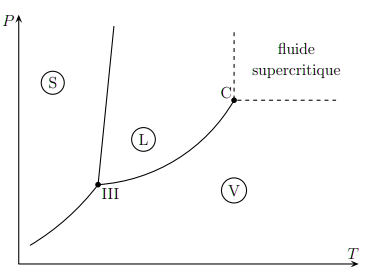
\includegraphics[width=0.5\linewidth]{../pic/3300/9.png}\\
    C : point critique .\\
    \rom{3} : point triple
\end{center}
\begin{itemize}
    \item Le point triple d'un corps pur est l'unique pression et l'unique température pour lesquelles le corps pur peut se trouver dans les trois phases simultanément.
    \item Le point critique d'un corps pur est l'unique pression et l'unique température au de là desquelles il n'y a plus de distinction possible entre liquide et solide.\\
          Lorsqu'un corps pur est dans un état tel que P > PC et TC alors il est dit être en phase
          fluide supercritique.

\end{itemize}
\subsection{Representation pression-volume-temperature}
\begin{center}
    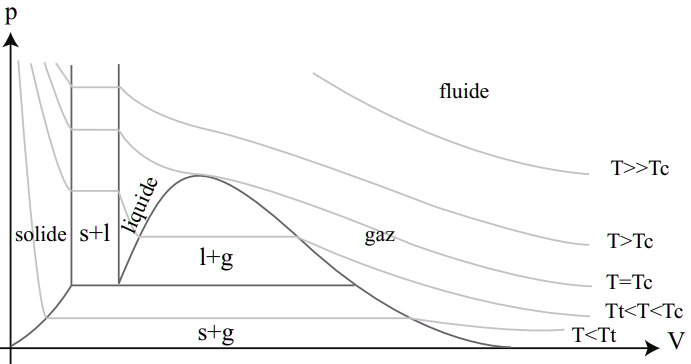
\includegraphics[width=0.5\linewidth]{../pic/3300/10.png}
    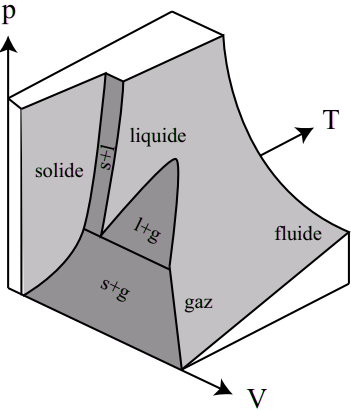
\includegraphics[width=0.2\linewidth]{../pic/3300/11.png}
\end{center}
\subsection{L'entropie}
Comme l'entropie est une mesure du désordre, elle croit lorsqu'on passe de la phase solide a la phase liquide et de la phase liquide a la phase gazeuse.
\begin{center}
    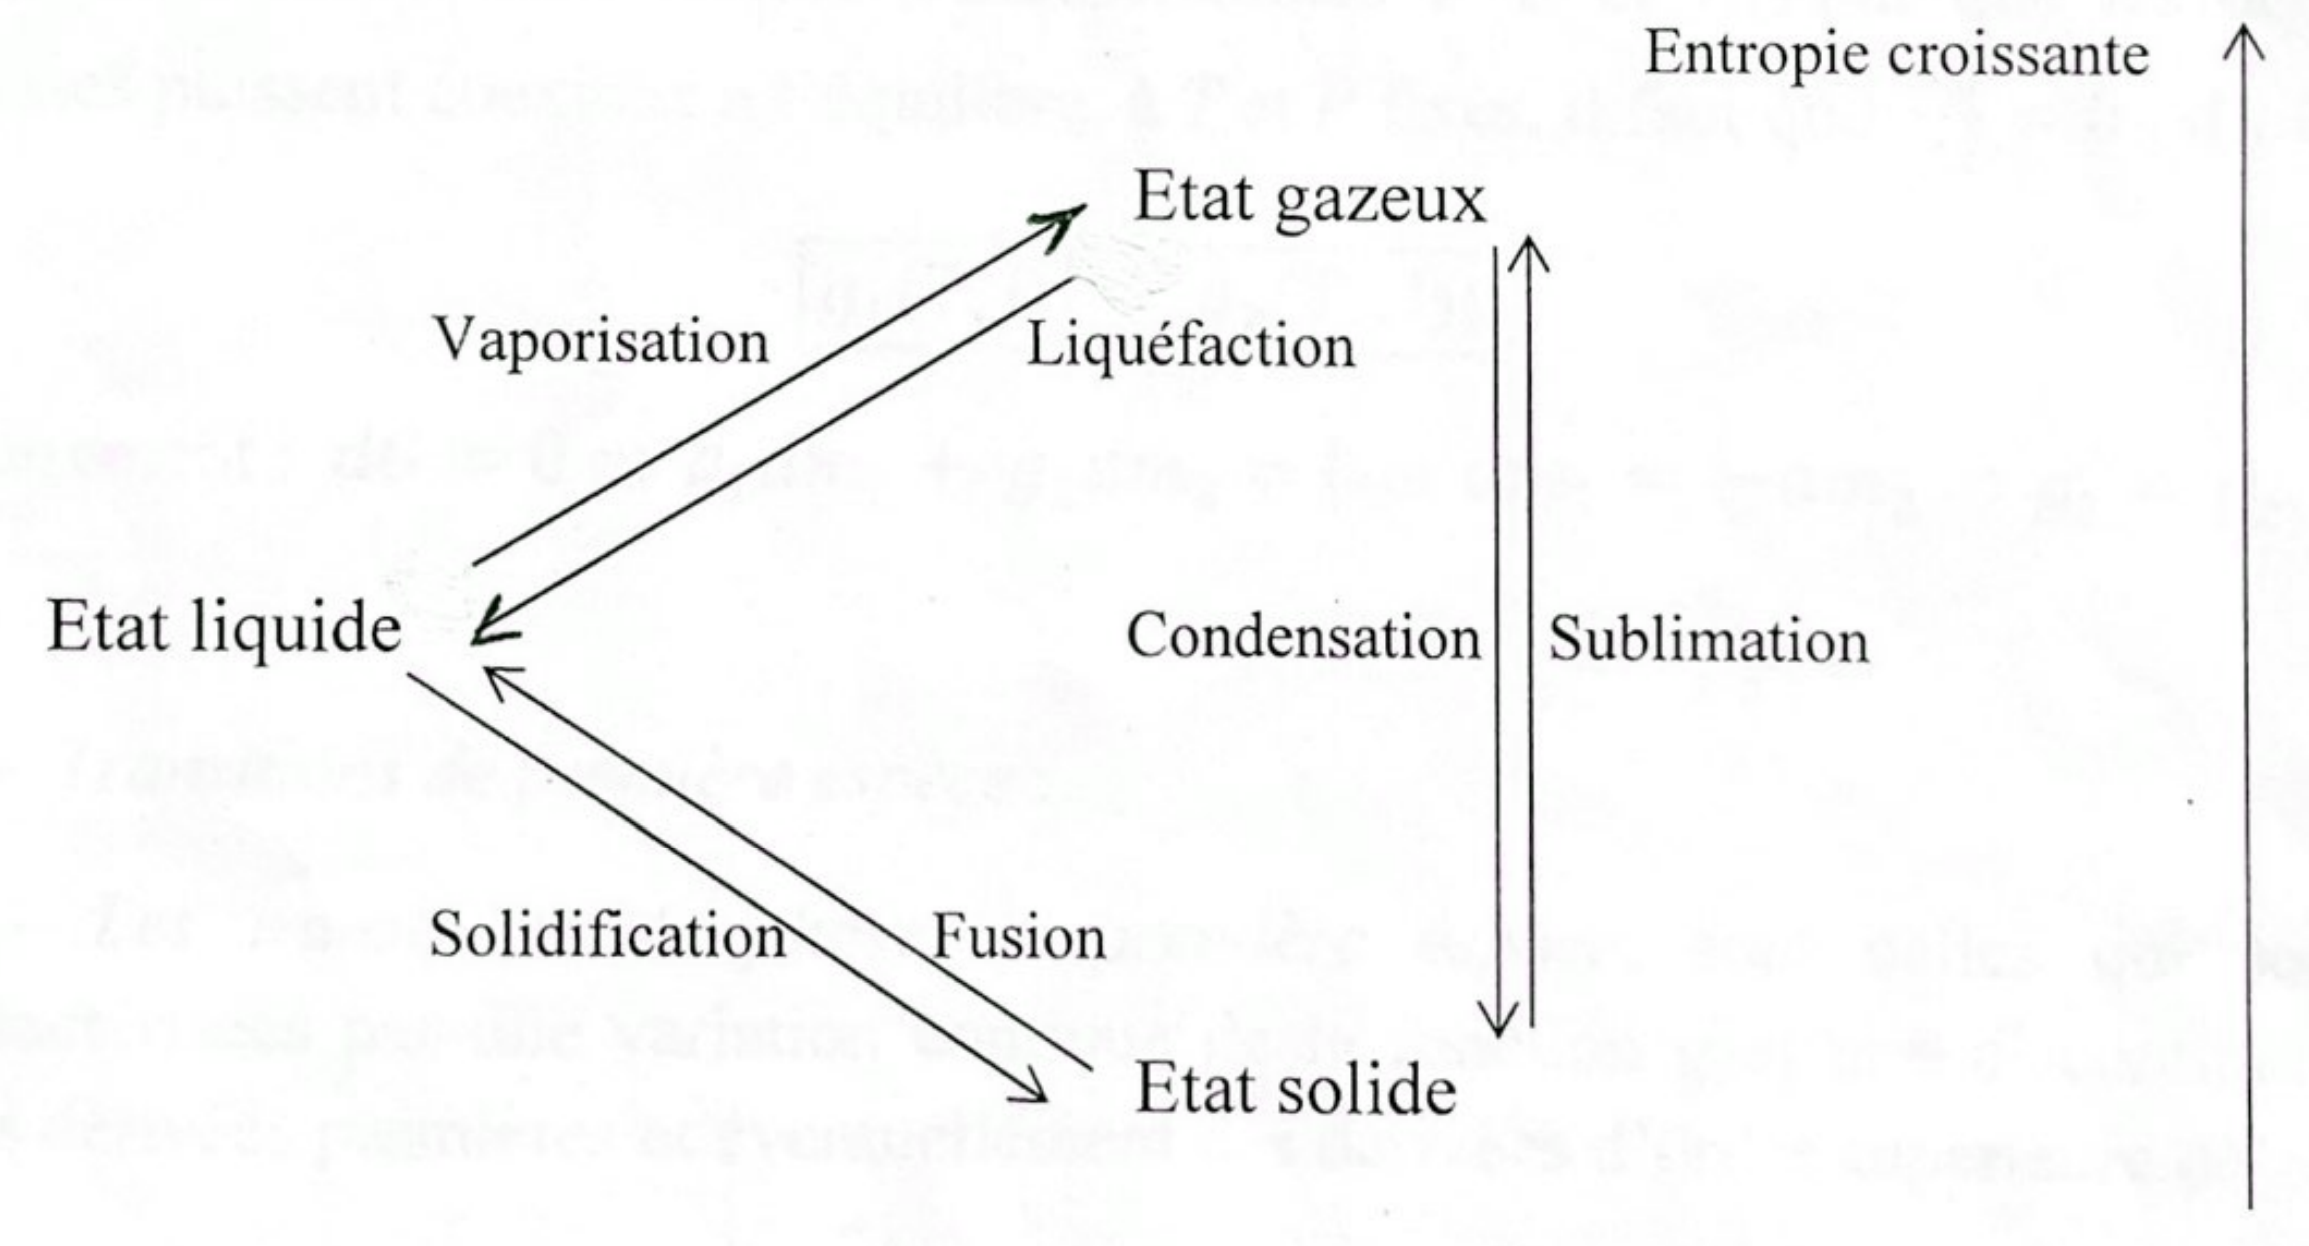
\includegraphics[width=0.5\linewidth]{../pic/3300/12.png}
\end{center}
\section{Équilibre d'un corps pur sous plusieurs phases}   
\subsection{Équilibre d'un corps pur sous deux phases}
    Pour que les deux phases puissent coexister a l’équilibre, a T et P fixes, il faut que :
    \[ g_1(T,P) = g_2(T,P) \]
\subsection{Transitions de premiere espèce}
    Les transitions de phase de premiere espèce, sont celles qui sont caractérisées par :
    \begin{itemize}
        \item une variation continue de la fonction $g$.
        \item une discontinuité des dérivées premieres et éventuellement des dérivées d'ordre supérieure de g.
    \end{itemize}
    $s $ et $v$ sont les dérivées d'ordre 1.\\
    $dg = -sdT + vdP \begin{cases}
        s = \frac{S}{m}\\
        v = \frac{V}{m}
    \end{cases} $
    Les dérivées d'ordre supérieur, telles que :
    \begin{itemize}
        \item la capacité thermique a $P = cte$:
            \[c_P =T (\frac{\partial s}{\partial T})_P = - T (\frac{\partial^2 g}{\partial T^2})_P\]
        \item le coefficient de compression isotherme :
            \[\mathbb{K}_T = - \frac{1}{v}(\frac{\partial v}{\partial P})_T = -\frac{1}{v}(\frac{\partial^2g}{\partial p^2})_T\]
        \item le coefficient de dilatation volumique:
            \[\alpha_v = \frac{1}{v}(\frac{\partial v}{\partial T})_P = \frac{1}{v}(\frac{\partial^2 g}{\partial P\partial T})_{T,P}\]
    \end{itemize}
\subsection{Chaleur latente}
    L'enthalpie massique de transition d'un corps pur $\Delta h_{12} = \frac{\Delta H_{12}}{m}$ de la phase 1 vers la phase 2.\\
    cette enthalpie massique est la chaleur latent $l_{12}$ pour réaliser la transition a temperature et une pression constantes.\\
    $l_{12} = \int\delta Q_p = \int dU + PdV = \int dU + d(PV) = \int dH$, et $\delta Q_p = TdS$ alors :
    \[ l_{12} = \Delta h_{12} = T \Delta s_{12} \]
\subsection{Formule de Clapeyron}
    Pour 2 états voisins d'un corps pur sous 2 phases on a les egalites suivant :\\
    $g_1(T,P) = g_2(T,P) \implies dg_1 = dg_2 \implies (\frac{\partial g_1 }{\partial P})_TdP + (\frac{\partial g_1}{\partial T})_PdT = (\frac{\partial g_2 }{\partial P})_TdP + (\frac{\partial g_2}{\partial T})_PdT$\\
    puisque $v = (\frac{\partial g}{\partial P})_T$ et $s = -(\frac{\partial g}{\partial T})_P \implies $.
    \[ \boxed{\frac{dP_{12}}{dT} = \frac{s_2-s_1}{v_2-v_1}} \]
\subsection{Transition de phase solid liquide}
    Lors d'un fusion l'entropie augmente, $\Delta h_f = T(v_L-v_S)\frac{dP_{sL}}{dT} > 0$ donne $v_L > v_S$ si $ \frac{dP_{sL}}{dT} > 0$, c'est le cas le plus frequent.\\
    lorsque $\frac{dP_{SL}}{dT} < 0$, ce qui est le cas de l'eau, on a $v_L < v_S$.
\subsection{Équilibre liquide-vapeur d'un corps pur}
Cette équation est obtenue en intégrant la formule de Clapeyron en supposant que l'enthalpie de vaporisation varie linéairement en fonction de la température. La formule de Dupré s'exprime selon :
\[\ln(P) = \alpha - \frac{\beta}{T}\]
\section{Transition de phase d'ordre élevé}
    \begin{itemize}
        \item l’enthalpie libre massique g et ses dérivées premiers (l'entropie massique s , v , etc.) sont des fonction continues
        \item Les dérivées d'ordre supérieur de g (ex:$C_p$), peuvent être discontinues.
    \end{itemize}
    Comme l'entropie massique ne varie pas, les transitions de phase d'ordre élevé sont cratérisées par l'absence de chaleur latente de transition.
    \begin{center}
        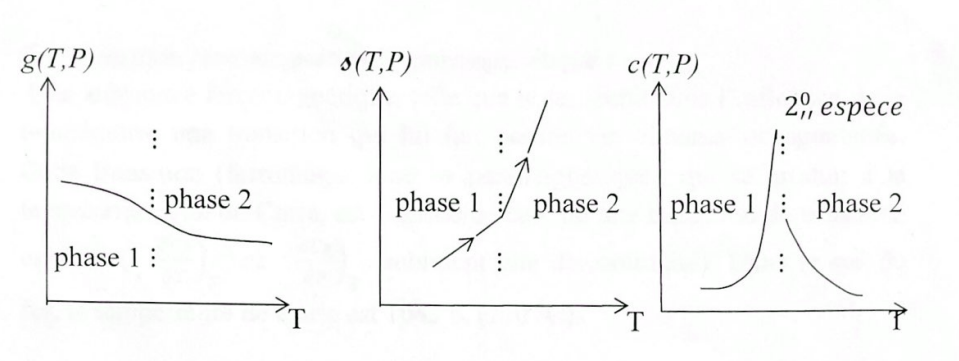
\includegraphics[width=0.5\linewidth]{../pic/3300/15.png}
    \end{center}
\subsection{Transition liquide-gaz au point critique}
    Un exemple de transition de phase de deuxième espèce, que l'on peut observer facilement, est la transition de phase liquide-gaz au point critique \\
    En ce point la relation de Clapeyron $\Delta h_{ij} = T(v_j-v_i)\frac{dP_{ij}}{dT}$ donne $\Delta h_{ij} = 0$ puisque $v_j = v_i$ et $\frac{dP_{ij}}{dT}$ est fini 
\subsection{Transition superfluide de l'helium liquide}
    La capacité thermique massique c du liquide helium \rom{1} augment considérablement lorsque la temperature diminue au voisinage de 2 K. En dessous de 2,17 K l'helium est un autre liquide: l'helium \rom{2}.
    Au cours de la transition de phase He \rom{1}$\to$ He \rom{2} , on ne constate aucune variation de volume,aucune enthalpie de transition , mais une discontinuité de $c \implies$ transition de phase de deuxième espèce 
\subsection{Transition conducteur-supraconducteur}
    En d’sous d'une certaine temperature de transition, la résistivité de certains solides s'effondre. Ils devienne supraconducteurs. En l'absence de champ magnétique applique, la transition a les caractères d'une transition de deuxième espèce:\\
    pas d'enthalpie de transition, mais une variation brutale de la capacité thermique a pression constante ($C_p$)\\
    Lorsque le matériau est soumis a un champ magnétique, la temperature de transition décroît et une enthalpie de transition apparaît: la transition de phase est alors de 1er espèce.
\subsection{Transition ferromagnétique-paramagnétique}
    Une substance ferromagnétique, telle que le fer subit sous l’influence de la temperature une transition que lui fait perdre son aimantation spontanée. \\
    Cette transition (ferromagnétique $\to$ paramagnétique), qui se produit a la temperature dite de Curie, est considérée comme un transition de troisième espèce $(\frac{\partial C_p}{\partial T})_p$ et $(\frac{\partial C_p}{\partial P})_T$ subissent une discontinuité. Dans le cas du fer, la temperature de Curie est $1043 K$

\end{document}